\documentclass[12pt]{article}
\usepackage{geometry}
\usepackage[spanish]{babel}
\geometry{margin=1in}
\usepackage{titlesec}
\usepackage{hyperref}
\usepackage{graphicx}
\usepackage{fancyhdr}
\pagestyle{fancy}
\fancyhf{}
\fancyhead[L]{\textbf{Documento de arquitectura}}
\fancyfoot[C]{\thepage}

% Title Section
\title{Documento de arquitectura \\
\large Sistema de comunicaciones seguras con segmentación virtual de dominios
}
\author{Alberto Daniel Lange}
\date{26 de febrero de 2025}

% Section Formatting
\titleformat{\section}{\large\bfseries}{\thesection}{1em}{}
\titleformat{\subsection}{\normalsize\bfseries}{\thesubsection}{1em}{}

\begin{document}

\maketitle
\begin{abstract}
    Este documento es una descripción, basada en el método Arcadia, de la arquitectura del dispositivo encriptador. Se describe la solución propuesta para cumplir con los requerimientos planteados en la documentación respectiva.
    \begin{center}
        v1.0
    \end{center}

\end{abstract}
\tableofcontents
\newpage

\section{Descripción de tecnologías}
En este apartado se describen las tecnologías a utilizar en el proyecto como propuesta de solución. 
\begin{itemize}
    \item \textbf{Noise Protocol Framework:} se trata de un marco para la creación de protocolos de comunicación seguros basado en el método Diffie-Hellmann. Permite especificar el procedimiento para la negociación de claves y la encriptación de mensajes utilizando combinaciones modulares de operaciones Diffie-Hellmann, funciones de hash y cifrados simétricos. Este framework es utilizado en sistemas de mensajería segura donde se requiere de cifrado extremo a extremo.
    
    \item \textbf{WireGuard:} WireGuard es un protocolo de túneles VPN derivado de Noise Protocol Framework. Está diseñado para ser simple, rápido y eficiente, proporcionando una solución de código abierto con una base de código pequeña, lo que ayuda a minimizar la superficie de ataque. Su propósito es proporcionar una alternativa segura y eficiente a los protocolos VPN tradicionales, permitiendo la creación de túneles seguros entre dispositivos en una red. 
    
    \item \textbf{seL4:} se trata de un microkernel con verificación formal matemática que garantiza que su implementación está libre de errores. Cuenta con una base de código muy reducida y proporciona un fuerte aislamiento entre procesos y una interfaz de comunicación segura. Es utilizado en sistemas críticos donde la seguridad y la confiabilidad son fundamentales. 
\end{itemize} 

\section{Arquitectura lógica}
% QUE ES LA ARQUITECTURA LÓGICA

Un hipervisor es un software que permite la creación y ejecución de múltiples máquinas virtuales, las cuales se ejecutan sobre hardware compartido de manera aislada e independiente. El hipervisor gestiona los recursos de hardware para cada máquina virtual según sea necesario, además provee una interfaz de comunicación entre las máquinas virtuales y el hardware.

El diseño propuesto está basado en la utilización de un hipervisor, el cual administra tres máquinas virtuales denominados dominios. En la figura \ref{fig:arquitectura_logica} se muestra un esquema de la arquitectura propuesta donde se presenta tanto la lógica interna del dispositivo a través de la interconexión de los dominios como la interacción con la red externa al encriptador.

\begin{figure}[h!]
    \centering
    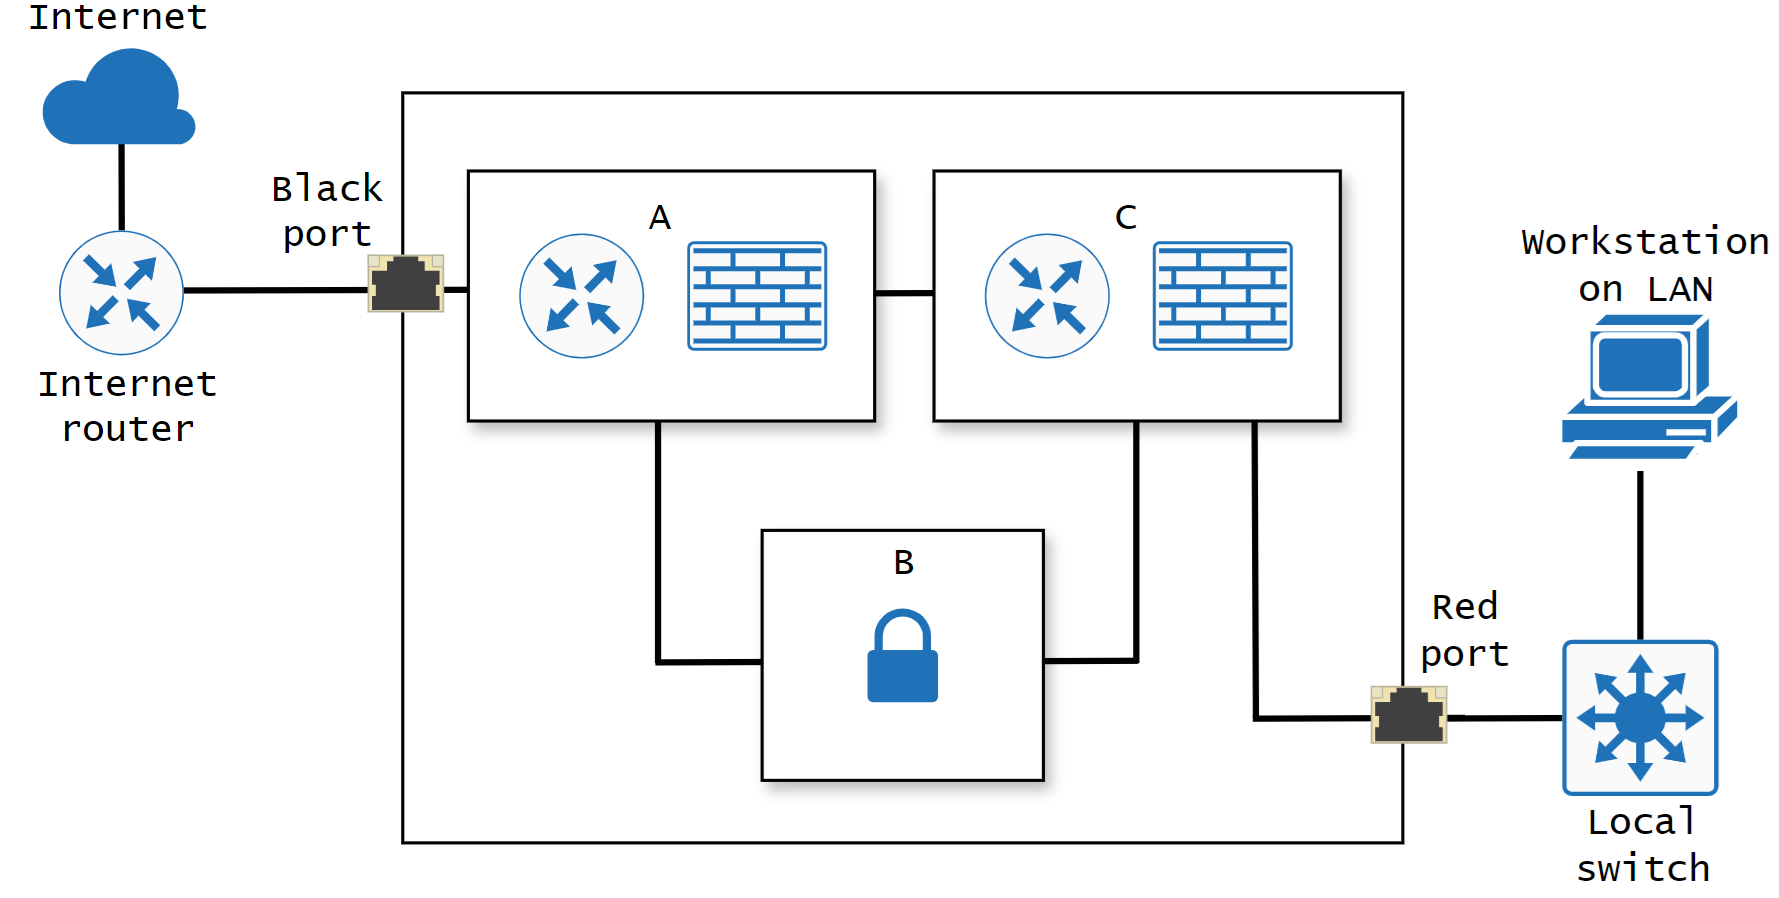
\includegraphics[width=0.75\textwidth]{images/arquitectura_logica.png}
    \caption{Esquema de arquitectura lógica del encriptador.}
    \label{fig:arquitectura_logica}
\end{figure}

\subsection{Dominio A - Negro}
El dominio A cuenta con tres interfaces de red, una física que lo conecta con el puerto de internet y dos virtuales que lo conectan con los dominios B y C.
Esta entidad actúa como primer firewall para el tráfico proveniente de internet y direcciona el tráfico hacia B o C según la dirección IP de origen de los paquetes. Si el tráfico proviene de otro sitio dentro de la red segura, este se direcciona hacia B para ser desencriptado. En el caso de ser tráfico proveniente de cualquier otro servicio de internet, este se direcciona hacia el dominio C.

\subsection{Dominio B - Encriptador}
Este dominio cuenta únicamente con dos interfaces virtuales, las cuales conectan a este dominio con A y C. Esta entidad administra el software necesario para el funcionamiento del túnel VPN, gestiona las claves para la conexión con otros nodos y realiza la encriptación/desencriptación de los paquetes salientes/entrantes respectivamente. Como base para la realización de estas funciones la entidad utiliza el software WireGuard.
La implementación de Wireguard requiere almacenar un par de claves pública y privada propios de cada nodo, además de la clave pública de demás nodos de la red. Estas claves son almacenadas en un archivo de configuración encriptado dentro de este dominio.

\subsection{Dominio C - Rojo}

Este dominio cuenta con una interfaz de red virtual que lo conecta con el dominio A y una interfaz física que lo conecta a la la red local del sitio. Esta entidad actúa como un segundo firewall para el tráfico proveniente de internet y direcciona el tráfico saliente hacia A o B según la dirección IP de destino de los paquetes provenientes de la red local. Si el tráfico tiene como destino un servicio de internet, este se direcciona hacia A, sin encriptación dedicada. En el caso de tener como destino otro sitio dentro de la red segura, este se direcciona hacia B para ser encriptado.


\end{document}